\sys is able to virtually merge tasks to construct a bigger virtual task and commit the state of the virtual task instead of the individual real tasks to improve execution time at stable energy supply environment. 

\begin{figure}
	\centering
	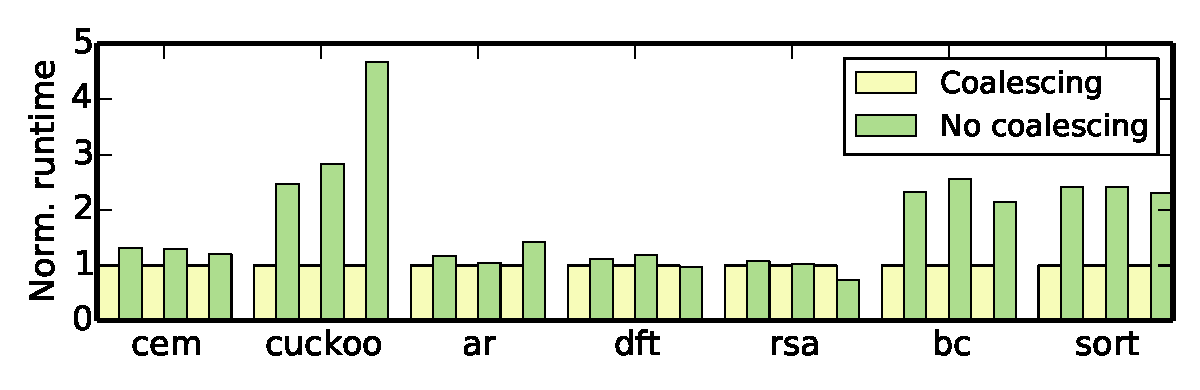
\includegraphics[width=\columnwidth]{figures/coalescing}
	\caption{This figure shows the performance of \sys when it uses the dynamic tasks coalescing mechanism as compared to its performance when the virtual task size is fixed to one, on multiple distances. }
	\label{fig:coalescing}
\end{figure}

\begin{figure}
	\centering
	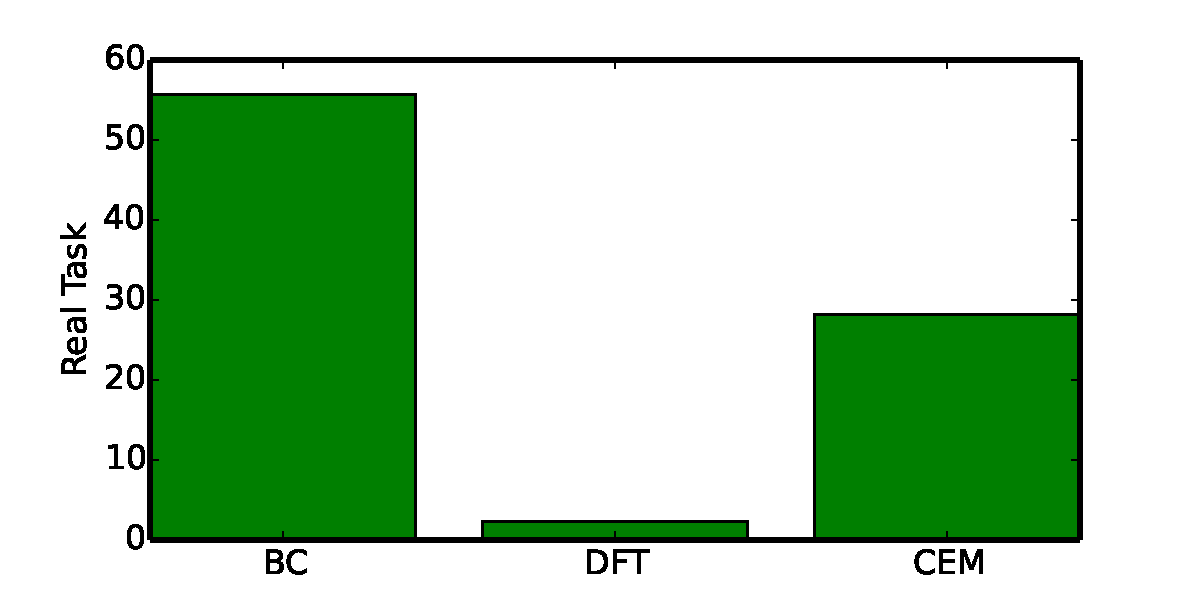
\includegraphics[width=\columnwidth]{figures/averageVirtualTaskSize}
	\caption{ This figure shows the average virtual task size (measured in real task unit) of the virtual task sizes that the coalescing algorithm used to accomplished the applications on a distance of 60cm. }
	\label{fig:aveVirtuTaskSize}
\end{figure}



\subsection{Task Merging Algorithm}

\begin{algorithm}[t]
	\caption{\sys task coalescing mechanism}
	\label{algorithm:coalescing_algorithm}
	\scriptsize
	\begin{algorithmic}[1]
		\State $\text{VT} \subset \{\sys~\text{tasks set}\}$  \Comment{Virtual task}
		\State $|\text{VT}|$ \Comment{VT size \todo{Define unit}{Amjad}}
		\State $\text{VT}_{\max}$ \Comment{Maximum VT size (With upper bound on coalescing)}
		\vspace{0.1cm}
		
		\While {True}
		\State $\text{VT} \leftarrow \text{VT}_{\text{next}}$ \Comment{\todo{Define $\text{VT}_{\text{next}}$}{Amjad}}
		\vspace{0.1cm}
		\While {execute VT} 
		\If { power failed $n$ times during task execution} \Comment{\todo{Define how it is detected}{Amjad}}				
		\State $|\text{VT}|:=|\text{VT}|-1$
		\State $\text{VT}_{\max} := |\text{VT}|$ \Comment{With upper bound on coalescing}
		\EndIf
		\EndWhile
		
		\vspace{0.1cm}
		\If {All tasks executed} \Comment{\todo{Define how it is detected and when}{Amjad}}
		\If{$|\text{VT}| < \text{VT}_{\max}$} \Comment{line added in fixed size approach}
		\State $|\text{VT}|:=|\text{VT}|+1$
		\EndIf
		\EndIf
		\EndWhile
	\end{algorithmic}
\end{algorithm}

The complete algorithm is provided in Algorithm~\ref{algorithm:coalescing_algorithm}. \todo{Fill in with missing information: scheduler description, implementation details, discussion}{Przemek/Amjad}

\subsection{Power Interrupt Immune Scheduler}

% TNT :  Total Number of Tasks
% JT 	: Total Jump
% ID	: Task ID
% D	: relative Jump (Delta)
% VCT_PT : Current Task Pointer

% if(TJ < TNT)
% 	VCT_PT <- VCT_PT + D
% else
% 	while ((dis = TJ - TNT) > TNT)
% 		dis -= ID
% 	VCT_PT <- VCT_PT + dis


\begin{algorithm}[t]
	\caption{\sys's scheduler: relative jump algorithm}
	\label{algo:relativeJump}
	\scriptsize
	%\small
	\begin{algorithmic}[1]
			\State \textsf{TNT}: Total Number of Tasks
			\State \textsf{ID}: Task ID
			\State \textsf{$\delta$}: Relative Jump
			\State $\textsf{TJ} \leftarrow (\textsf{ID} + \delta )$ \Comment{Total Jump}
			\State \textsf{\textsf{$VCT_{pt}$}}: Virtual Current Task Pointer

			\If { \textsf{TJ} > \textsf{TNT} }
				\State $\textsf{dis} = \textsf{TJ} - \textsf{TNT}$
				\While{ $ \textsf{dis} > TNT $ }
					\State $\textsf{dis} -= \textsf{TNT}$
				\EndWhile
				\State $\textsf{dis} -= \textsf{ID}$
				\State \textsf{$VCT_{pt}$} $+= \textsf{dis}$
			\Else
				\State \textsf{$VCT_{pt}$} $+= \delta $

			\EndIf
	\end{algorithmic}
\end{algorithm} %Task jumping algorithm

It utilizes a persistent circular buffer (i.e. persistent linked list) to keep the state of a program across power failures. \sys provides an API to enable a programmer to have a full control over the execution flow of the program, i.e. (un)blocking a task or re-execute the same task which is particularly important in the intermittent execution to emulate a persistent loop. \todo{Expand this section}{Amjad}

\begin{figure}
	\centering
	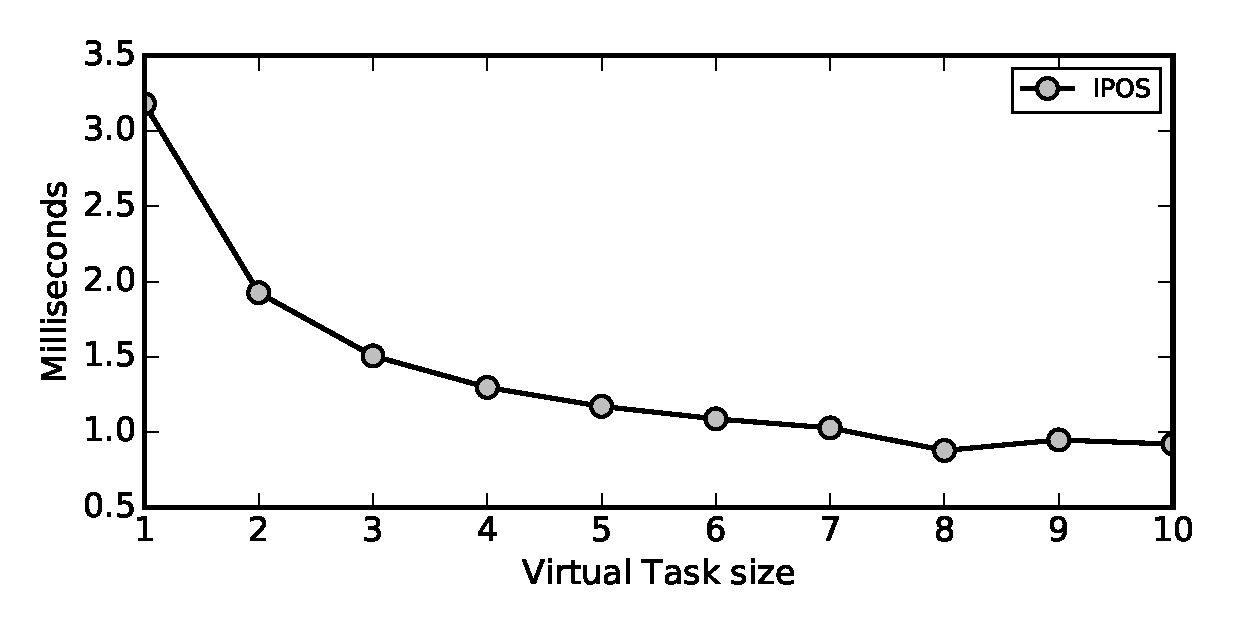
\includegraphics[width=\columnwidth]{figures/virtualTaskSize.eps}
	\caption{Execution time of a dummy application containing twelve empty tasks as a function of coalescing factor. We observe three times improvement from coalescing until four virtual tasks, while we observe a diminishing return from task coalescing beyond four. \todo{Improve the figure: make it narrower, larger font, remove legend, do not capitalize "Task" in X axis, add Y axis label (Execution time (ms))}{Amjad}}
	\label{fig:virtualTaskSize}
\end{figure}

The question remains: does coalescing all program's tasks into a singe virtual task (as the energy becomes fully available, i.e. from energy harvesting to continuous power environment) is the best one?. To answer this question we have implemented a simple program composed of $x$ empty tasks. We execute the same program by increasing coalescing factor by one while the device on which the program was executed was running on a stable power supply (refer to Section~\ref{sec:methodology_evaluation} for details). The result is presented in Figure~\ref{fig:virtualTaskSize}. We observe a significant increase in execution time as task are coalescent from one to four (three times execution time improvement). However, as the coalescing increases beyond four, we observe diminishing returns from coalescing in terms of execution time. \todo{Decide whether to place this figure in Evaluation section or leave it here}{Przemek}

%\begin{algorithm}
%	\caption{Opportunistic virtual Task size}
%	\label{algo:fixVirtTask}
%	\scriptsize
%	%\small
%	\begin{algorithmic}[1]
%		\State $VT \subset \text{\{\sys Tasks\}} $  \Comment{$VT:$ Virtual Task}
%		\State VTS : VT size
%		\vspace{0.1cm}
%		
%		\While {$True$}
%		\State $VT \leftarrow VT_{next}$
%		\vspace{0.1cm}
%		\While {execute $VT$} 
%		\If { $\text{power failed twice}$ }				
%		\State $VTS--$  
%		\EndIf
%		\EndWhile
%		
%		\vspace{0.1cm}
%		\If {$ \text{All tasks executed}$}
%		\State $VTS++$
%		\EndIf
%		\EndWhile
%	\end{algorithmic}
%\end{algorithm}